\section{Approach}
\label{sec:approach}
\begin{wrapfigure}[13]{l}{45mm}
\centering
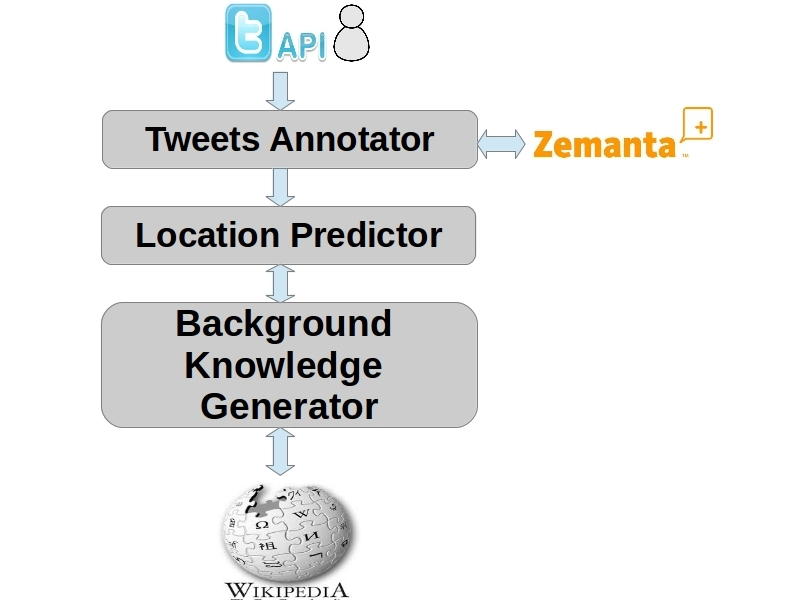
\includegraphics[width = 5cm]{images/architecture-2.jpg}
%\vspace*{-0.75em}
\caption{Architecture}
\label{fig:architecture}
\end{wrapfigure}
\vspace*{-1.00em}
Previous research~\cite{bo2012geolocation,cheng2010you} have established that the content of a user's posts reflects his/her geographical location. Using the same intuition we propose an approach that uses Wikipedia as the background knowledge. An overview of the approach is shown in Figure~\ref{fig:architecture}. It comprises of three components \begin{inparaenum}[(1)]\item Tweets Annotator: Extracts Wikipedia entities from a user's tweets, \item Background Knowledge Generator: Generates background knowledge for each city using Wikipedia \item Location Predictor: Utilizes the output of \textit{Tweets Annotator} with \textit{Background Knowledge} to predict the location of the user. \end{inparaenum} 
%We propose to use the information available in Wikipedia to establish entities that are most representative of a given location. Wikipedia is a large encyclopedia containing dedicated pages for cities. Proportional to the size of the city, it Wikipedia page generally contains a variety of information about the city like it geography, culture, sports team, cityscape etc. Our hypothesis is that by correlating the occurrence of city specific entities from Wikipedia in a user's tweets, we can estimate the location of the user

%\subsection{Dataset} (This should go to the Evaluation section)
%We randomly selected 600 users containing 1000+ tweets each, from the dataset made publicly available by Cheng et al\cite{cheng2010you}. Our dataset has users from 48 states across US. 
\subsection{Annotation of Users' Tweets}
Derczynski et.al, in their latest work~\cite{derczynski2013} have compared three state of art \textit{entity recognition and linking} systems for tweets. The systems compared with corresponding \textit{Precision, Recall and F-Measures} are \begin{inparaenum} \item Dbpedia Spotlight~\cite{mendes2011dbpedia} (P=20.1, R=47.4, F=28.3), \item Zemanta\footnote{\url{http://developer.zemanta.com/}} (P=57.5, R=31.8, F=\textbf{41.0}) and \item TextRazor\footnote{\url{http://www.textrazor.com/technology}} (P=\textbf{64.6}, R=26.9, F=38.0) \end{inparaenum}. We used Zemanta\footnote{\url{http://developer.zemanta.com/docs/suggest/}} because of its relatively superior performance and also because of their rate limit extension (10,000 per day) provided for research purposes, on request\footnote{We thanks Zemanta for their support.}. 

\subsection{Creation of Background Knowledge}
Wikipedia is a large encyclopedia containing dedicated pages for geographical locations. Proportional to the size of the location, its Wikipedia page generally contains a variety of information about the place like its geography, culture, sports team, cityscape etc.

Links to internal Wikipedia pages from a given page are an important feature of all Wikipedia pages. The aim of these links is to increase the understanding of a user about the given page. For instance, the Wikipedia page of \textit{Boston, Massachusetts} \footnote{http://en.wikipedia.org/wiki/Boston} mentions the \textit{Boston Red Sox}, in the Sports section. It also provides a hyperlink to Boston Red Sox, that allows the user to navigate to the Wikipedia page of \textit{Boston Red Sox}. We base our approach on the assumption that these internal links share varying degrees of relevance to the Wikipedia page of the city. As in the previous example, the Wikipedia page of Boston also contains an internal link to \textit{Major League Baseball} which would be less representative of Boston than the \textit{Boston Red Sox}. 

To create our knowledgebase, we selected 1670 cities in the United States of America having population greater than 20000. The entire collection of Wikipedia is available for download\footnote{http://en.wikipedia.org/wiki/Wikipedia:Database\_download}. We use the dump dated 14-Feb-2014 to extract the internal links from the Wikipedia pages of all the cities in our dataset. Figure 1 shows the distribution of the count of internal links among all the city pages. From our dataset, \textit{Pittsburgh} had 2684 as the largest count of internal links and \textit{Round Lake Beach, Illinois} had 33 as the smallest count of internal links.

\subsubsection{Scoring city-specific Entities}
Given a set of internal links for a city, we score each link to determine the degree of its relevance to the city. The more a given internal link is common to the cities in our dataset, the less it maybe relevant to one particular city. For example, in our dataset of 1650 cities, an internal link to the Wikipedia page of \textit{Barack Obama} appears 105 times as opposed to \textit{Southern California} and \textit{Golden Gate Bridge} which appear 50 and 6 times respectively. 

Mendes et al. \cite{mendes2011dbpedia} proposed \textit{Inverse Candidate Frequency} for the task of entity disambiguation in DBPedia Spotlight. The idea behind ICF is that "a word commonly co-occuring with many resources is less discriminative overall". We use this intuition to identify the discriminative ability of an internal link with respect to a city. Let C be the set of cities in our dataset. Let I be the set of internal links for a city c $\in$ C. The ICF of an internal link i $\in$ I, that appears in \textit{n} cities, is defined as:
\begin{equation}
	ICF(i) = \log |C|- \log n
\end{equation}

\subsection{Location Estimation}
We used Zemanta\footnote{http://www.zemanta.com} to annotate tweets. It maps entities in the input text to Wikipedia pages.

For a user U, let $T_{u}$ be the set of their tweets, $Z_{u}$ = \{$z_{1}$,$z_{2}$,...,$z_{k}$\} be the set of entities annotated by Zemanta that map to a Wikipedia url. Let |$z_{k}$| represent the cardinality $z_{k}$ in $T_{u}$. Let C be the set of cities in out dataset and $\forall$ $c_{j}$ $\in$ C, let $L$ be the set of its internal wiki links where \textit{ICF}($l_{i}$) is the score $\forall$ $l_{i}$ $\in$ L.

For the user U we compute the score of each city in our set as:
\begin{equation}
	Score(c_{j}) = \sum_{i=1}^I |l_{i}| \times ICF(l_{i})\qquad  \forall l_{i} \in Z_{u}
\end{equation}

We tag the city with the maximum score as the location of the user. (PAVAN: User argmax/argmin here -- make it more a mathematical notation).




